\documentclass{book}
\usepackage{physics}
\usepackage{graphicx}
\usepackage{caption}
\usepackage{amsmath}
\usepackage{authblk}
\usepackage{amsfonts}
\usepackage{esint}
\usepackage{mathtools}
\usepackage{amsthm}
\theoremstyle{definition}
\newtheorem{defn}{Definition}[section]
\newtheorem{prop}{Proposition}[section]
\newtheorem{rmk}{Remark}[section]
\newtheorem{thm}{Theorem}[section]
\newtheorem{exmp}{Example}[section]
\newtheorem{prob}{Problem}[section]
\newtheorem{sln}{Solution}[section]
\newtheorem*{prob*}{Problem}
\newtheorem{exer}{Exercise}[section]
\newtheorem*{exer*}{Exercise}
\newtheorem*{sln*}{Solution}
\usepackage{empheq}
\usepackage{hyperref}
\usepackage{tensor}
\usepackage{xcolor}
\hypersetup{
	colorlinks,
	linkcolor={black!50!black},
	citecolor={blue!50!black},
	urlcolor={blue!80!black}
}
\newcommand{\p}{\partial}
\newcommand{\R}{\mathbb{R}}
\newcommand{\C}{\mathbb{C}}
\newcommand{\lag}{\mathcal{L}}

\newcommand{\ham}{\mathcal{H}}

\newcommand{\I}{\mathcal{I}}
\newcommand{\K}{\mathcal{K}}
\newcommand{\F}{\mathcal{F}}
\newcommand{\w}{\omega}
\newcommand{\lam}{\lambda}
\newcommand{\al}{\alpha}
\newcommand{\be}{\beta}
\newcommand{\x}{\xi}

\newcommand{\f}[2]{\frac{#1}{#2}}

\newcommand{\ift}{\infty}

\newcommand{\lp}{\left(}
\newcommand{\rp}{\right)}

\newcommand{\lb}{\left[}
\newcommand{\rb}{\right]}

\newcommand{\lc}{\left\{}
\newcommand{\rc}{\right\}}


\newcommand{\V}{\mathbf{V}}
\newcommand{\U}{\mathcal{U}}
\newcommand{\Id}{\mathcal{I}}


%\setcounter{chapter}{-1}


\makeatletter
\renewcommand{\@chapapp}{Part}
%\renewcommand\thechapter{$\bf{\ket{\arabic{chapter}}}$}
%\renewcommand\thesection{$\bf{\ket{\arabic{section}}}$}
%\renewcommand\thesubsection{$\bf{\ket{\arabic{subsection}}}$}
%\renewcommand\thesubsubsection{$\bf{\ket{\arabic{subsubsection}}}$}
\makeatother



\usepackage{subfig}
\usepackage{listings}
\captionsetup[lstlisting]{margin=0cm,format=hang,font=small,format=plain,labelfont={bf,up},textfont={it}}
\renewcommand*{\lstlistingname}{Code \textcolor{violet}{\textsl{Mathematica}}}
\definecolor{gris245}{RGB}{245,245,245}
\definecolor{olive}{RGB}{50,140,50}
\definecolor{brun}{RGB}{175,100,80}
\lstset{
	tabsize=4,
	frame=single,
	language=mathematica,
	basicstyle=\scriptsize\ttfamily,
	keywordstyle=\color{black},
	backgroundcolor=\color{gris245},
	commentstyle=\color{gray},
	showstringspaces=false,
	emph={
		r1,
		r2,
		epsilon,epsilon_,
		Newton,Newton_
	},emphstyle={\color{olive}},
	emph={[2]
		L,
		CouleurCourbe,
		PotentielEffectif,
		IdCourbe,
		Courbe
	},emphstyle={[2]\color{blue}},
	emph={[3]r,r_,n,n_},emphstyle={[3]\color{magenta}}
}


\begin{document}
\begin{titlepage}\centering
 \clearpage
 \title{{\textsc{\textbf{QUANTUM\\ Mechanics, Optics, and Information}}}\\ \smallskip - A Quick Guide - \\}
 \author{\bigskip Huan Q. Bui}
  \affil{Colby College\\$\,$\\ PHYSICS \& MATHEMATICS\\ Statistics \\$\,$\\Class of 2021\\}
 \date{\today}
 \maketitle
 \thispagestyle{empty}
\end{titlepage}

\subsection*{Preface}
\addcontentsline{toc}{subsection}{Preface}

Greetings,\\

This text is my reading notes from Shankar's \textit{Principles of Quantum Mechanics, Second Edition}, \textit{Introductory Quantum Optics} by , \textit{Optical Coherence \& Quantum Optics}. Additional comes from my class notes, my comments/interpretations/solutions, and other books/articles/notes. There are three parts to this text, as the title suggests. The Quantum Mechanics part covers the principles of quantum mechanics. A majority of this part will be my reading notes from Shankar's book. The other two topics parts cover selected phenomena in quantum optics and quantum information theory.  \\

Background in linear algebra will be very helpful. I will try to cover some of the mathematical background, but a lot of familiarity will be assumed. \\

Enjoy!

\newpage
\tableofcontents
\newpage





\chapter{QUANTUM MECHANICS}


\newpage


\section{Mathematical Introduction}

\subsection{Linear Vector Spaces}

We should familiar with defining characteristics of linear vector spaces at this point. Here are some important definitions/theorems again:

\begin{defn}
	A linear vector space $\textbf{V}$ is a collection of objects called \textit{vectors} for which there exists
	
	\begin{enumerate}
		\item A definite rule for summing, and
		\item A definite rule for scaling, with the following features:
		
		
		\begin{itemize}
			\item Closed under addition: for $x,y \in \V$, $x+y \in \V$.
			\item Closed under scalar multiplication: $x\in \V$, then $ax \in \V$ for some scalar $a$.
			\item Scalar multiplication is distributive. 
			\item Scalar multiplication is associative.
			\item Addition is commutative.
			\item Addition is associative.
			\item There exists a (unique) null element in $\V$.
			\item There exists a (unique) additive inverse. 
		\end{itemize}
	\end{enumerate}
\end{defn}


Vector spaces are defined over some field. The field can be real numbers, complex numbers, or it can also be finite. As for good practice, we will begin to label vectors with Dirac bra-ket notation. So, for instance, $\ket{v} \in \V$ denotes vector $v \in \V$. Basic manipulations of these vectors are intuitive:
\begin{enumerate}
	\item $\ket{0}$ is unique, and is the null element.
	\item $0\ket{V} = \ket{0}$.
	\item $\ket{-V} = -\ket{V}$.
	\item $\ket{-V}$ is a unique additive inverse of $\ket{V}$.
\end{enumerate} 

The reasons for choosing to use the Dirac notation will become clear later on. Another important basic concept is \textit{linear (in)dependence}. Of course, there are a number of equivalent statement for linear independence. We shall just give one here:

\begin{defn}
	A set of vectors is said to be linearly independent if the only linear relation 
	\begin{align}
	\sum^n_{i=1}a_i\ket{i} = \ket{0}
	\end{align}
	is the trivial one where the components $a_i = 0$ for any $i$. 
\end{defn}



The next two basic concepts are \textit{dimension} and \textit{basis}. 

\begin{defn}
	A vector space $\V$ has dimension $n$ if it can accommodate a maximum of $n$ linearly independent vectors. We denote this $n$-dimensional vector space as $\V^n$.
\end{defn}

We can show that 

\begin{thm}
	Any vector $\ket{v} \in \V^n$ can be written (uniquely) as a linear combination of any $n$ linearly independent vectors.  
\end{thm}


\begin{defn}
	A set of $n$ linearly independent vectors in a $n$-dimensional space is called a \textit{basis}. So if $\ket{1},\dots,\ket{n}$ form a basis for $\V^n$, then any $\ket{v}\in \V$ can be written uniquely as
	\begin{align}
	\ket{v} = \sum^n_{i=1}a_i\ket{i}.
	\end{align}
\end{defn}

It is nice to remember the following:
\begin{align}
\boxed{\text{Linear Independence} = \text{Basis} + \text{Span}}
\end{align}

When a collection of vectors span a vector space $\V$, it just means that any $\ket{v} \in \V$ can be written as a linear combination of (some of) these vectors. 


The algebra of linear combinations is quite intuitive. If $\ket{v} = \sum_i a_i\ket{i}$ and $\ket{w} = \sum_i b_i\ket{i}$ then 

\begin{enumerate}
	\item $\ket{v + w} = \sum_i (a_i + b_i)\ket{i}$.
	\item $c\ket{v} = c\sum_i a_i\ket{i} = \sum_i ca_i\ket{i}$.
\end{enumerate}



A linear algebra text will of course provide a much better coverage of these topics. 















\subsection{Inner Product Spaces}


A generalization of the familiar dot product is the \textit{inner product} or the \textit{scalar product}. An inner product between two vectors $\ket{v}$ and $\ket{w}$ is denoted $\braket{v|w}$. An inner product has to satisfy the following properties:

\begin{enumerate}
	\item Conjugate symmetry (or skew-symmetry):$\braket{v}{w} = \braket{w}{v}^*$.
	\item Positive semi-definiteness: $\braket{v}{v} \geq 0$.
	\item Linearity in ket: $\braket{v}{aw + bz} = a\braket{v}{w} + b\braket{v}{z}$.
	\item Conjugate-linearity in bra: $\braket{av + bz}{w} = \bar{a}\braket{v}{w} + \bar{b}\braket{z}{w}$.
\end{enumerate}




\begin{defn}
	An inner product space is a vector space with an inner product. 
\end{defn}


\begin{defn}
	$\innerproduct{v}{w} = 0 \iff \ket{v} \perp \ket{w}$. 
\end{defn}


\begin{defn}
	The \textit{norm} (or length) of $\ket{v}$ is defined as 
	\begin{align}
	\norm{v} = \sqrt{\braket{v}}.
	\end{align}
	Unit vectors have unit norm. Unit vectors are said to be \textit{normalized}.  
\end{defn}




\begin{defn}
	A set of basis vectors all of unit norm, which are pairwise orthogonal will be called an \textit{orthonormal basis} or ONB. 
\end{defn}


Let $\ket{v} = \sum_i a_i\ket{i}$ and $\ket{w} = \sum_i b_i \ket{j}$, then 
\begin{align}
\braket{v}{w} = \sum_i a_i^*b_i \braket{i}{j}.
\end{align}



\begin{thm}
	\textbf{Gram-Schmidt:} Given a linearly independent basis, we can form linear combinations of the basis vectors to obtain an orthonormal basis. 
\end{thm}

Suppose that the Gram-Schmidt process gives us an ONB then we have
\begin{align}
\braket{i}{j} = \delta_{ij}.
\end{align}
As a result,
\begin{align}
\braket{v}{w} = \sum_i v_i^*w_i.
\end{align}
Alternatively, we can think this as doing the standard inner products of vectors whose entries are the components of the vectors $\ket{v}$, $\ket{w}$ in the basis:
\begin{align}
\ket{v} \to \begin{bmatrix}
v_1\\v_2\\\vdots\\v_n
\end{bmatrix}\hspace{0.5cm}
\ket{w} \to \begin{bmatrix}
w_1\\w_2\\\vdots\\w_n
\end{bmatrix} \implies \braket{v}{w} = \begin{bmatrix}
v_1^* & v_2^* & \dots & v_n^*
\end{bmatrix}\begin{bmatrix}
w_1\\ w_2 \\\vdots \\ w_n
\end{bmatrix}.
\end{align}
We can also easily see that 
\begin{align}
\braket{v}{v} = \sum_i \abs{v_i}^2 \geq 0.
\end{align}

\subsection{Dual Spaces and Dirac Notation}
Here we deal with some technical details involving the \textit{ket} (the column vectors) and the \textit{bra} (the row vectors). Column vectors are concrete manifestations of an abstract vector $\ket{v}$ in a basis, and we can work backward to go from the column vectors to the kets. We can do a similar thing with the bra vectors - since there's nothing special about writing the entries is a column versus in a row. However, we will do the following. We know that associated with every ket $\ket{v}$ is a column vector. So let its adjoint, which is a row vector, be associated with the bra, called $\bra{v}$. Now, we have two vector spaces, the space of kets and the dual space of bras. There is a basis of vectors $\ket{i}$ for expanding kets and a similar basis $\bra{i}$ for expanding bras. 

\subsubsection{Expansion of Vectors in an ONB}
It is extremely useful for us to be able to express a vector in an ONB. Suppose we have a vector $\ket{v}$ in an ONB $\ket{i}$. Then, let $\ket{v}$ be written as
\begin{align}
\ket{v} = \sum_i v_i \ket{i}.
\end{align}
To find the components $v_i$, we take the inner product of $\ket{v}$ with $\ket{j}$:
\begin{align}
\braket{j}{v} = \sum_i v_i \braket{j}{i} = \sum_i v_i\delta_{ij} = v_j.
\end{align}
With this, we can rewrite the vector $\ket{v}$ in the basis $\ket{i}$ as
\begin{align}
\ket{v} = \sum_i \ket{i}\braket{i}{v}.
\end{align}



\subsubsection{Adjoint Operations}
Here is a few details regarding taking the adjoints of vectors. Suppose that
\begin{align}
\ket{v} = \sum_i v_i\ket{i} = \sum_i \ket{i}\braket{i}{v}.
\end{align}
Then,
\begin{align}
\bra{v} = \sum_i\ket{i}v_i^*.
\end{align}
Now, because $v_i = \braket{i}{v}$, we have $v_i^* = \braket{v}{i}$. Thus, 
\begin{align}
\bra{v} = \sum_i \braket{v}{i}\bra{i}.
\end{align}
In plain words, the rule for taking the adjoint is the following. To take the adjoint of an equation involving bras and kets and coefficients, reverse the order of all factors, exchanging bras and kets and complex conjugating all coefficients. 


\subsubsection{Gram-Schmidt process}
Again, the Gram-Schmidt process lets us convert a linearly independent basis into an orthonormal one. For a two-dimensional case, procedure is the following:
\begin{enumerate}
	\item Rescale the first by its own length, so it becomes a unit vector. This is the first (orthonormal) unit vector.
	\item Subtract from the second vector its projection along the first, leaving behind only the part perpendicular to the first. (Such a part will remain since by assumption the vectors are nonparallel).
	\item Rescale the left over piece by its own length. We now have the second basis vector: it s orthogonal to the first and of unit length.
\end{enumerate}

In general, let $\ket{I}, \ket{II}, \dots$ be a linearly independent basis. The first vector of the orthonormal basis will be
\begin{align}
\ket{1} = \f{\ket{I}}{\norm{\ket{I}}}.
\end{align}
For the second vector in the basis, consider
\begin{align}
\ket{2'} = \ket{II} - \ket{1}\braket{1}{II}.
\end{align}
We can see that $\ket{2'}$ is orthogonal to $\ket{1}$:
\begin{align}
\braket{1}{2'} = \braket{1}{II} - \braket{1}\braket{1}{II} = 0.
\end{align}
So dividing $\ket{2'}$ by its norm gives us, $\ket{2}$, the second element in the ONB. To find the third element in the ONB, we have to first make sure it is orthogonal to both $\ket{I}$ and $\ket{II}$, so let us consider
\begin{align}
\ket{3'}= \ket{III} - \ket{1}\braket{1}{III} - \ket{2}\braket{2}{III}.
\end{align}
Once again we have $\ket{3'}$ orthogonal to both $\ket{1}$ and $\ket{2}$. Normalizing $\ket{3'}$ gives us $\ket{3}$, the third element in the ONB. We can now see how this process continues to the last element. 



\subsubsection{Schwarz and Triangle Inequality}
Just two small yet very important details:
\begin{thm}
	Schwarz Inequality:
	\begin{align}
	\abs{\braket{v}{w}} \leq \norm{v}\norm{w}
	\end{align}
\end{thm}


\begin{thm}
	Triangle Inequality:
	\begin{align}
	\norm{v+w} \leq \norm{v} + \norm{w}.
	\end{align}
\end{thm}



\subsection{Subspaces, Sum and Direct Sum of Subspaces}
I'm not too happy with the definitions given by Shankar's book. He also uses the notation for direct sum to indicate vector space addition, which is very confusing. Any linear algebra textbook would provide better definitions. For equivalent statements about directness of vector space sums, check out my \href{https://huanqbui.com/LaTeX\%20projects/Matrix_Analysis/HuanBui_MatrixAnalysis.pdf}{Matrix Analysis} notes. 




\subsection{Linear Operators}
Again, a rigorous definition of an operator can be found in almost any linear algebra textbook. But here,we can simply think of an operator as just some linear transformation from a vector space to itself. Say, if $\Omega$ is some operator that sends $\ket{v}$ to $\ket{v'}$, we write
\begin{align}
\Omega\ket{v} = \ket{v'}.
\end{align}
By definition, $\ket{v}$ and $\ket{v'}$ are contained in the same vector space. Now, we note that $\Omega$ can also act on bras:
\begin{align}
\bra{v}\Omega = \bra{v'}.
\end{align}
But of course the order of writing things is different, and once again, $\bra{v}$ and $\bra{v'}$ are contained in the same (dual) space. 


Next, because $\Omega$ is linear, we have the following familiar rules:
\begin{align}
\Omega \alpha \ket{v_i} &= \alpha\Omega \ket{v_i}.\\
\Omega \{ \alpha \ket{v_i} + \beta\ket{v_j} \} &= \alpha\Omega\ket{v_i} + \beta\Omega \ket{v_j}.\\
\bra{v_i}\alpha\Omega &= \bra{v_i}\Omega \alpha\\
\{\bra{v_i}\alpha + \bra{v_j}\beta \}\Omega &= \alpha\bra{v_i}\Omega + \beta \bra{v_j}\Omega.
\end{align}


One of the nice features of linear operators is that the action of an operator is completely determined by what it does to the basis vectors. Suppose 
\begin{align}
\ket{v} = \sum_i v_i \ket{i}
\end{align}
and 
\begin{align}
\Omega\ket{i} = \ket{i'},
\end{align}
then
\begin{align}
\Omega \ket{v} = \sum_i \Omega v_i \ket{i}= \sum_iv_i \Omega\ket{i} = \sum_iv_i\ket{i'}.
\end{align}



The next point of interest is \textit{products} of operators. As we might have seen, operators don't always commute. A product of operators applied to a vector just means operators are applied in sequence. The \textit{commutator} of two operators $\Omega, \Lambda$ is defined as
\begin{align}
\Omega\Lambda - \Lambda\Omega \equiv \lb \Omega,\Lambda \rb.
\end{align}
In general, $\lb \Omega,\Lambda\rb$ is not zero. Suppose three operators $\Omega, \Lambda, \Theta$ are involved, then we have two useful relations:
\begin{align}
&\lb \Omega, \Lambda\Theta \rb = \Lambda\lb \Omega, \Theta \rb + \lb \Omega, \Lambda \rb \Theta\\
&\lb \Lambda\Omega, \Theta \rb = \Lambda\lb \Omega, \Theta \rb + \lb \Lambda, \Theta \rb \Omega.
\end{align}
We notice that the form resembles the chain rule in calculus. 





\subsection{Matrix Elements of Linear Operators}
One thing we will hear very often in quantum mechanics is the idea of matrix elements. The idea, it turns out, is very simple. Suppose we have a basis $\ket{i}$, and an operator $\Omega$ such that
\begin{align}
\Omega\ket{i} = \ket{i'}.
\end{align}
Then, for
\begin{align}
\ket{v} = \sum_i v_i \ket{i}, 
\end{align}
we have
\begin{align}
\Omega\ket{v} = \Omega \sum_i v_i \ket{i} = \sum_i v_i \Omega\ket{i} = \sum_i v_i \ket{i'}.
\end{align}
Because we know $\Omega$ and $\ket{i}$, $\ket{i'}$ is also known, as in its components in the basis $\ket{j}$ (un-primed) are known:
\begin{align}
\braket{j}{i'} = \bra{j}\Omega\ket{i} \equiv \Omega_{ji},
\end{align}
where the $n^2$ numbers $\Omega_{ji}$ are the matrix elements of $\Omega$ in this basis. Now, if
\begin{align}
\Omega\ket{v} = \ket{v'}
\end{align}
then the components of the transformed ket $\ket{v'}$ can be expressed in terms of the components of $\ket{v}$ and the matrix elements $\Omega_{ji}$:
\begin{align}
v_i' = \braket{i}{v'} = \bra{i}\Omega\ket{v} = \bra{i}\Omega \sum_j v_j \ket{j} = \sum_j v_j \bra{i}\Omega\ket{j} = \sum_j \Omega_{ij}v_j.
\end{align}
We can see the above equation in matrix form as well:
\begin{align}
\begin{bmatrix}
v_1'  \\ \vdots \\ v_n'
\end{bmatrix}
=
\begin{bmatrix}
\bra{1}\Omega\ket{1} &  \dots & \bra{1}\Omega\ket{n} \\
\vdots & \ddots & \vdots\\	
\bra{n}\Omega\ket{1} & \dots & \bra{n}\Omega\ket{n} \\
\end{bmatrix}
\begin{bmatrix}
v_1 \\ \vdots \\ v_n 
\end{bmatrix}.
\end{align}
The elements of the first column are simply the components of the first transformed basis vector $\ket{1'} = \Omega\ket{1}$ in the given basis. Likewise, the elements of the j$^{\text{th}}$ column represent the image of the j$^\text{th}$ basis vector after $\Omega$ acts on it. 


\subsection{Matrix Elements of Products of Operators}

To get the matrix elements of a product of two operators, we do the following. Suppose we have operators $\Omega$ and $\Lambda$, then
\begin{align}
(\Omega\Lambda)_{ij} = \bra{i}\Omega\Lambda\ket{j} = \bra{i}\Omega \mathcal{I} \Lambda \ket{j}.
\end{align}
Now, we observe that 
\begin{align}
\mathcal{I} = \sum_k \ket{k}\bra{k}. 
\end{align}
So, 
\begin{align}
(\Omega \Lambda)_{ij} = \sum_k \bra{i}\Omega\ket{k}\bra{k}\Lambda \ket{j} = \sum_k \Omega_{ik}\Lambda_{kj}.
\end{align}



\subsection{The Adjoint of an Operator}
Recall that for a scalar $\alpha$
\begin{align}
\bra{\alpha v} = \bra{v}\alpha^*,
\end{align}
then we have a similar thing with operators if
\begin{align}
\Omega\ket{v} = \ket{v'}
\end{align}
then 
\begin{align}
\bra{\Omega v} = \bra{v}\Omega^\dagger,
\end{align}
where $\Omega^\dagger$ is \textit{the} adjoint of $\Omega$. The relationship between $\Omega^\dagger$ and $\Omega$ can be seen in a basis. We consider the matrix elements of $\Omega^\dagger$ in a basis:
\begin{align}
(\Omega^\dagger)_{ij} = \bra{i}\Omega^\dagger \ket{j} = \bra{\Omega i}\ket{j} = \bra{j}\ket{\Omega i}^* = \bra{j} \Omega \ket{i}^* = \Omega_{ji}^*.
\end{align}
We see that
\begin{align}
\Omega^\dagger_{ij} = \Omega^*_{ji},
\end{align}
i.e., in matrix form, $\Omega^\dagger$ is the conjugate transpose of $\Omega$. 

The rule for taking adjoins of equations is rather simple: When a product of operators, bras, kets, ad explicit numerical coefficients is encountered, reverse the order of all factors and make the substitution $\Omega \leftrightarrow \Omega^\dagger$, $\ket{} \leftrightarrow \bra{}$, $a \leftrightarrow a^*$. 


\subsection{Hermitian, Anti-Hermitian, and Unitary Operators}

\begin{defn}
	An operator $\Omega$ is Hermitian $\iff \Omega = \Omega^\dagger$.
\end{defn}


\begin{defn}
	An operator $\Omega$ is anti-Hermitian $\iff \Omega = -\Omega^\dagger$.
\end{defn}

Shankar's book ignores a bigger class of operators called \textit{normal} operators. Normal operators commute with their adjoints. In a sense, normal operators act \textit{like numbers}. Hermitian (or self-adjoint) operators are a subset of normal operators. So, the number-likeness of normal operators carries over to Hermitian operators and anti-Hermitian operators as well. Hermitian and anti-Hermitian operators are like pure real and pure imaginary numbers. Just as every number maybe be decomposed into a sum of pure real and pure imaginary parts, it turns out that we can decompose every operator into its Hermitian and anti-Hermitian parts. 
\begin{align}
\Omega = \f{\Omega + \Omega^\dagger}{2} + \f{\Omega - \Omega^\dagger}{2}.
\end{align}
One can verify that the first terms is Hermitian, and the second term is anti-Hermitian. 




\begin{defn}
	An operator $\mathcal{U}$ is unitary $\iff \mathcal{U}\mathcal{U}^\dagger = \mathcal{I}$. 
\end{defn}

Unitary operators are like complex numbers of unit modulus. 


\begin{thm}
	Unitary operators preserves the inner product between the vectors they act on.
	\begin{proof}
		Suppose
		\begin{align}
		\ket{v'} &= \mathcal{U}\ket{v}\\
		\ket{w'} &= \mathcal{U}\ket{w}.
		\end{align}
		Then
		\begin{align}
		\braket{v'}{w'} = \braket{\mathcal{U}v}{\mathcal{U}w} = \bra{v}\mathcal{U}^\dagger\mathcal{U}\ket{w} = \braket{v}{w}.
		\end{align}
	\end{proof}
\end{thm} 



\begin{thm}
	The columns (or rows) of a unitary matrix form an ONB.
	\begin{proof}
		Refer to a linear algebra text. The key is to consider an inner product between any two columns/rows.
	\end{proof}
\end{thm}


\subsection{Active and Passive Transformation}

Suppose all $\ket{v}$ is unitarily transformed to $\ket{v'}$:
\begin{align}
\ket{v} \to \U \ket{v}.
\end{align}
Then under this transformation, the matrix elements of any operator $\Omega$ are modified as follows:
\begin{align}
\ket{v'}\Omega\ket{v} \to \ket{\U v'} \Omega \ket{\U v} = \bra{v'}\U^\dagger \Omega \U \ket{v}.
\end{align}
It is clear that the same change is equivalent to leaving the vectors alone and subjecting all operators to the change
\begin{align}
\Omega \to \U^\dagger \Omega \U.
\end{align}

\textit{Active transformation} refers to changing the vectors, while \textit{passive transformation} refers to changing the operators.





\subsection{The Eigenvalue Problem}
I won't say much about what eigenvectors and eigenvalues are because we should be familiar with these concepts at this point. But just to introduce some terminology, each operator has certain kets of its own called \textit{eigenkets}, on which its action is simply that of scaling. So, eigenkets are just a different word for eigenvectors of an operator:
\begin{align}
\Omega\ket{v} = \omega\ket{v}.
\end{align}

Shankar's book talks about the characteristic equation and characteristic polynomial. While these are legitimate ways to find eigenvalues and eigenvectors, it is often very difficult. I'd prefer Leo Livshits' and Sheldon Axler's way and use minimal polynomials instead. I would steer away from determinants and characteristic polynomials at this point. 


\begin{thm}
	Eigenvalues of a Hermitian operator are real. 
	\begin{proof}
		Suppose 
		\begin{align}
		\Omega\ket{w} = a\ket{w},
		\end{align}
		then
		\begin{align}
		\bra{w}\Omega\ket{w} = a\braket{w},
		\end{align}
		and thus
		\begin{align}
		a^* \braket{w} = \bra{w}\Omega^\dagger\ket{w} = \bra{w}\Omega\ket{w} = a\braket{w}.
		\end{align}
		So we have
		\begin{align}
		(a - a^*)\braket{w} = 0.
		\end{align}
		Because $\ket{w}$ are eigenkets, they are cannot be the zero vector. This means $a = a^*$.
	\end{proof}
\end{thm}


Some might worry about the existence of eigenvalues of Hermitian operators. But worry no more, because Hermitian operators are a subclass of normal operators, which are a subclass of diagonalizable operators. This simply says Hermitian matrices are diagonalizable, and all its eigenvalues are real. But it turns out there is a little bit more to this. 


\begin{thm}
	For every Hermitian operator $\Omega$, there exists an ONB comprised entirely of the eigenvectors of $\Omega$. 
\end{thm}

Once again, this should be no surprise if one has studied normal operators. Hermitian operators inherit this property from its normalness. This property of normal operators are called the Spectral Theorem (for normal operators, of course). The proof of all this can be found in many linear algebra texts. 


\begin{thm}
	The eigenvalues of a unitary operator are complex numbers of unit modulus. 
	\begin{proof}
		The key to the proof is using inner products. 
	\end{proof}
\end{thm}



\subsubsection{Simultaneous Diagonalization of Two Hermitian Operators}

I would say the topic of simultaneous diagonalizability is covered quite well in Leo Livshits' course and hence in my \href{https://huanqbui.com/LaTeX\%20projects/Matrix_Analysis/HuanBui_MatrixAnalysis.pdf}{Matrix Analysis} notes. But here I will just give the most important results. 

\begin{thm}
	If $\Omega$ and $\Lambda$ are two commuting Hermitian operators, there exists a basis of common eigenvectors that diagonalizes them both. 
\end{thm} 

This result is not too surprising if we have studied simultaneous diagonalizability before. A more general theorem says that 
\begin{align}
\text{Simultaneous diagonalizbility} \iff \text{Individual diagonalizability} + \text{Commutativity}.
\end{align}
It is clear that because all Hermitian operators are diagonalizable, if two Hermitian operators commute, they are simultaneously diagonalizable.



\subsubsection{The Propagator}

In quantum mechanics (and classical mechanics of course), it is quite common to have some final state vector be obtained from an initial state vector multiplied by some matrix, which is independent of the initial state. We call this matrix the \textit{propagator}. 


The central problem in quantum mechanics is finding the state of a quantum system $\ket{\psi}$, which obeys the Schr\"{o}dinger equation:
\begin{align}
i\hbar \ket{\dot{\psi}} = J\ket{\psi}
\end{align}
where the Hermitian operator $H$ is called the \textit{Hamiltonian}. We will see much more of this as we move on.



\subsection{Functions of Operators and Related Concepts}


In this section, we look at whether it makes sense to define functions of operators. We will only restrict ourselves to functions that can be written as a power series. Consider a series
\begin{align}
f(x) = \sum_{n=0}^\infty = a_n x^n
\end{align}
where $x$ is a scalar. We defined the same function of an operator to be
\begin{align}
f(\Omega) = \sum_{n=0}^\infty a_n\Omega^n.
\end{align}
Now, this definition only makes sense if we have convergence. Consider this example:
\begin{align}
e^\Omega = \sum^\infty_{n=0}\f{\Omega^n}{n!},
\end{align}
where $\Omega$ is Hermitian. In the eigenbasis of $\Omega$, $\Omega$ is diagonal. This means we can add and/or take powers of $\Omega$ by add and/or take powers of the diagonal entries. We can find that
\begin{align}
e^\Omega = \begin{bmatrix}
\sum^\infty_{m=0}\f{\omega^m_1}{m!}&&\\
&&\\
&&\sum^\infty_{m=0}\f{\omega^m_n}{m!}
\end{bmatrix}
\end{align}
where $\omega_i$ are the eigenvalues of $\Omega$. We note that each entry in the expression above converges to $e^{\omega_i}$.



\subsubsection{Derivatives of Operators with Respect to Parameters}
Now, consider some operator $\Theta(\lambda)$ that depends on a parameter $\lambda$. The derivative of $\Theta$ with respect to $\lambda$ is defined to be
\begin{align}
\f{d\Theta(\lambda)}{d\lambda} = \lim_{\Delta\lambda \to 0} \lb \f{\Theta(\lambda + \Delta \lambda) - \Theta(\lambda)}{\Delta \lambda} \rb.
\end{align}
If $\Theta(\lambda)$ is written as a matrix, then the matrix of $d\Theta/d\lambda$ is obtained by differentiating the matrix elements of $\Theta(\lambda)$. A case that might be interesting to us is 
\begin{align}
\Theta(\lambda) = e^{\lambda\Omega}.
\end{align}
It turns out that if $\Omega$ is Hermitian or ``nice enough'' then 
\begin{align}
\f{d\Theta(\lambda)}{d\lambda} = \Omega e^{\lambda\Omega} = e^{\lambda\Omega}\Omega = \Theta(\lambda)\Omega = \Omega \Theta(\lambda).
\end{align}
Conversely, if we have
\begin{align}
\f{d\Theta(\lambda)}{d\lambda} = \Theta(\lambda)\Omega
\end{align}
then 
\begin{align}
\Theta(\lambda) = ce^{\lambda\Omega}
\end{align}
where $c$ is some operator. But we have to be careful that $c$ might not commute with $e^{\lambda\Omega}$.

The business of whether two operators commute or don't can make things slightly more complicated. If $\Theta$ and $\Omega$ commute, i.e., $[\Theta, \Omega] = 0$, then the rules of exponentiation carries over very nicely:
\begin{align}
&e^{a\Omega}e^{b\Omega} = e^{(a + b)\Omega}\\
&e^{a\Omega}e^{b\Theta} = e^{a\Omega + b\Theta}\\
&e^{a\Omega}e^{b\Theta}e^{-a\Omega} = e^{b\Theta}.
\end{align}
If $[\Omega, \Theta] \neq 0$, then the second and third equations no longer hold. Likewise, in differentiating a product, we have to be extra careful:
\begin{align}
\f{d}{d\lambda}e^{\lambda\Omega}e^{\lambda\Theta} = \Omega e^{\lambda\Omega}e^{\lambda\Theta} + e^{\lambda\Omega}e^{\lambda\Theta}\Theta.
\end{align}
While $[\Omega, e^{\lambda\Omega}] = 0$, because $\Theta$ and $\Omega$ might not commute, we can't bring $\Omega$ over to the right of $e^{\lambda\Theta}$. 


\subsection{Generalization to Infinite Dimensions}


\subsubsection{The Dirac delta function}
Consider the ordered $n$-tuple $\{ f_n(x_1), \dots, f_n(x_n) \}$ as components of a ket $\ket{f_n}$ in a vector space $\V^n(\mathbb{R})$:
\begin{align}
\ket{f_n} \leftrightarrow \begin{bmatrix}
f_n(x_1) \\ \vdots \\ f_n(x_n)
\end{bmatrix}.
\end{align}
The basis vectors in this space are:
\begin{align}
\ket{x_i} \leftrightarrow \begin{bmatrix}
0 \\ 0 \\ \vdots \\ 1 \\ 0 \\ \vdots \\ 0
\end{bmatrix} \leftarrow i^{th} \text{place}.
\end{align}
The basis vectors satisfy \textit{orthogonality} and \textit{completeness}:
\begin{align}
&\braket{x_i}{x_j} = \delta_{ij}\\
&\sum_{i=1}^n \ket{x_i}\bra{x_i} = \Id.
\end{align}
With this,
\begin{align}
\ket{f_n} = \sum_{i=1}^n f_n(x_i)\ket{x_i}.
\end{align}
We next define the inner product in this space:
\begin{align}
\braket{f_n}{g_n} \ sum^n_{i=1}f_n(x_i)g_n(x_i).
\end{align}
The functions $f_n$ and $g_n$ are said to be orthogonal if $\braket{f_n}{g_n} = 0$. We also have that
\begin{align}
\braket{f_n}{f_n} = \sum^n_{i=1}[f_n(x_i)]^2.
\end{align}
For finite $n$, nothing ``bad'' can really happen here. But what if $n$ is infinity? What we need is the redefinition of the inner product for finite $n$ in such a way that as $n$ goes to infinity, we get a smooth limit. A natural choice is
\begin{align}
\braket{f_n}{g_n} = \sum^n_{i=1} f_n(x_i)g_n(x_i)\f{L}{n+1}
\end{align}
where $L$ is the length of the interval. If we now let $n$ go to infinity, we get
\begin{align}
&\braket{f}{g} = \int^L_0 f(x)g(x)\,dx\\
&\braket{f} = \int^L_0 f^2(x)\,dx.
\end{align}
Now, if we consider complex functions as well in some interval $a\leq x \leq b$, the inner product becomes:
\begin{align}
\braket{f}{g} = \int^b_a f^*(x)g(x)\,dx.
\end{align}
But what are the basis vectors in this space and are they normalized? We know that 
\begin{align}
\braket{x}{x'} = 0
\end{align}
if $x \neq x'$. But what if $x = x'$? It turns out that we cannot simply require $\braket{x}{x} = 1$. The best way to see this is to deduce the correct normalization. We start with the completeness relation:
\begin{align}
\int^b_a \ket{x'}\bra{x'}\,dx' = \Id. 
\end{align}
Now, consider this
\begin{align}
\int^b_a \braket{x}{x'}\braket{x'}{f}\,dx' = \bra{x}\Id \ket{f} = \braket{x}{f}.
\end{align}
This is nothing but the projection of $\ket{f}$ along the basis ket $\ket{x}$, which is just $f(x)$. So, we also have $f(x') = \braket{x'}{f}$. Let the inner product $\braket{x}{x'}$ be some unknown function $\delta(x,x')$. Since $\delta(x,x')$ vanishes if $x\neq x'$, we can restrict the integral to an infinitesimal region near $x'=x$. With these, the equality above gives
\begin{align}\label{delt}
\int^{x+\epsilon}_{x-\epsilon}\delta(x,x')f(x')\,dx' = f(x).
\end{align}
In this infinitesimal region, $f(x)$ can assumed to be constant, and thus can be pulled out of the integral, leaving
\begin{align}
f(x)\int^{x+\epsilon}_{x-\epsilon} \delta(x,x')\,dx' = f(x).
\end{align}
And so we have
\begin{align}
\int^{x+\epsilon}_{x-\epsilon} \delta(x,x')\,dx' = 1. 
\end{align}
Clearly, $\delta(x,x')$ cannot be finite at $x=x'$. It should be infinite in such a way that its integral is 1. Since $\delta(x,x')$ depends only on the difference $x-x'$, we can write it as $\delta(x-x')$. So, the function $\delta(x-x')$ has the properties:
\begin{align}
\begin{cases}
\delta(x-x') = 0, \hspace{0.5cm} x \neq x'\\
\int^b_a \delta(x-x')\,dx' = 1\hspace{0.5cm} a < x < b
\end{cases}.
\end{align}
This is called the \textbf{Dirac delta function} and it fixes the normalization of the basis vectors:
\begin{align}
\braket{x}{x'} = \delta(x-x').
\end{align}

The Dirac delta function is ``strange'' in the sense that its value is either zero or infinite. It's thus useful to view it as the limit of a Gaussian:
\begin{figure}[!htb]
	\centering
	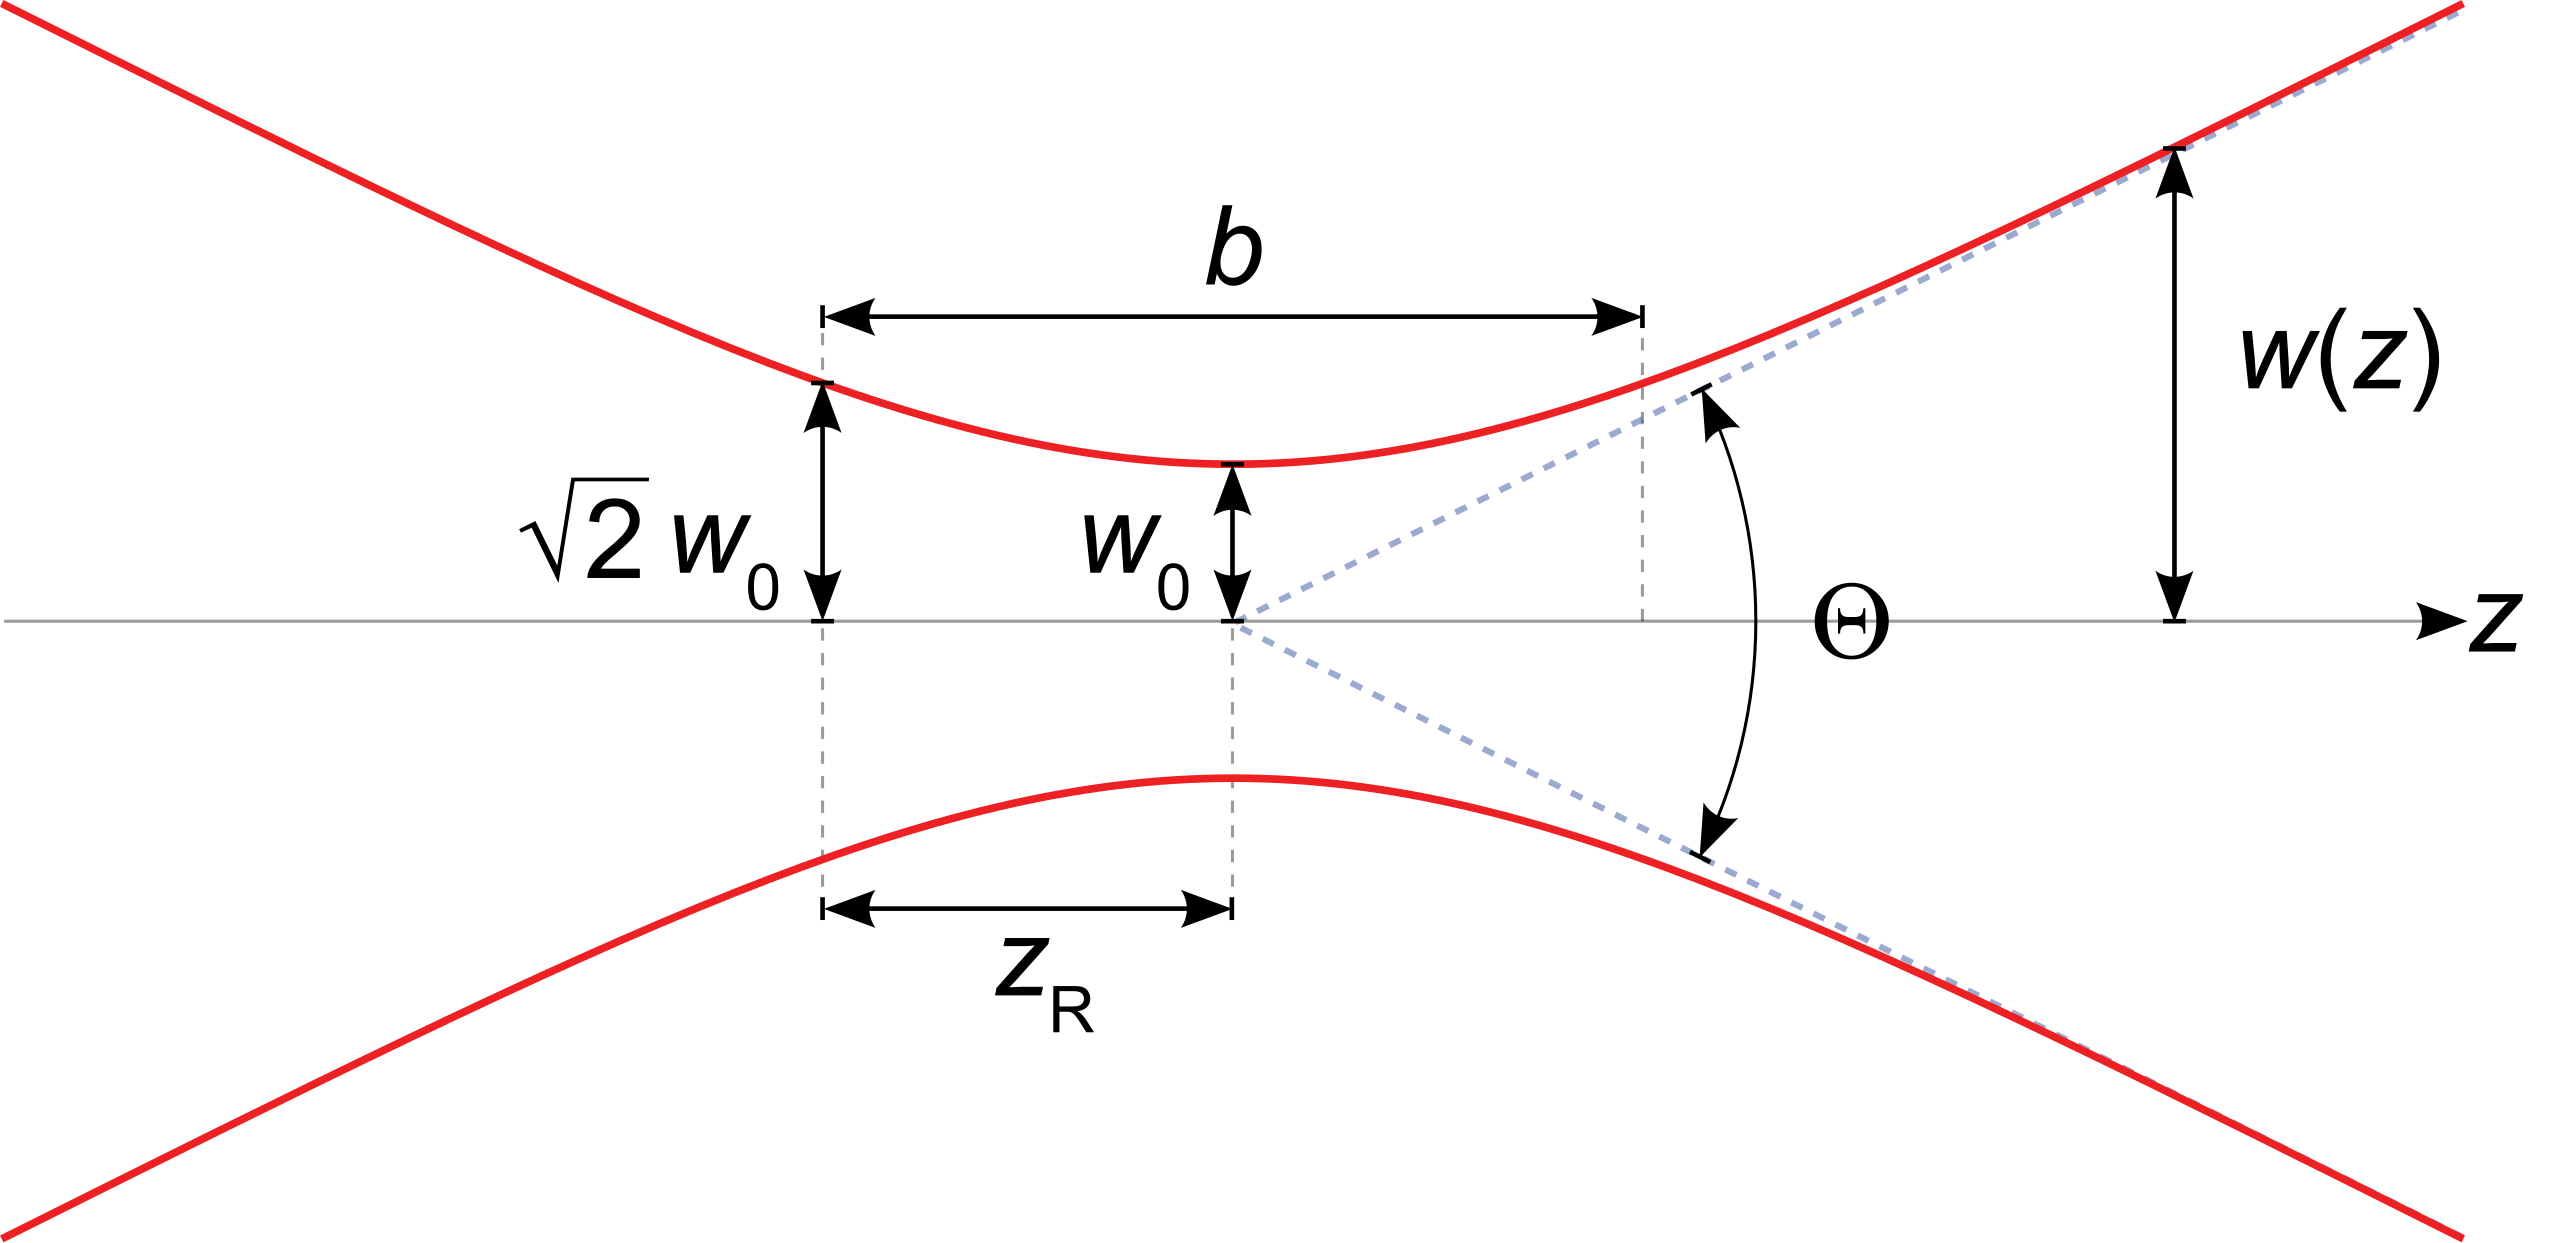
\includegraphics[scale=0.3]{gauss.png}
\end{figure}

of the form
\begin{align}
g_\Delta(x-x') = \f{1}{\sqrt{\pi \Delta^2}}e^{-(x-x')^2/\Delta^2}.
\end{align}
It is clear that the area under the curve is one (one can easily check this). Also, $\Delta \to 0$, $g_\Delta$ becomes closer and closer to $\delta(x-x')$ (the area under the curve is the same, while the width of the peak becomes smaller and smaller). 


From Gaussian model, we know that the delta function is not only real but also even:
\begin{align}
\delta(x-x') = \delta(x'-x).
\end{align}
Next, we consider the derivative of $\delta(x-x')$ with respect to $x$:
\begin{align}
\delta'(x-x') = \f{d}{dx}\delta(x-x') = -\f{d}{dx'}\delta(x-x').
\end{align}
Once again, we consider the Gaussian model. We consider $dg_\Delta(x-x')/dx = -dg_\Delta(x-x')/dx'$ as a function of $x'$:
\begin{figure}[!htb]
	\centering
	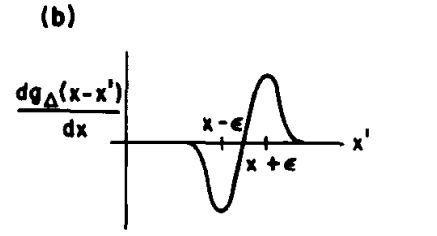
\includegraphics[scale=0.5]{dgauss.png}
\end{figure}

As $g_\Delta$ shrinks,, each bump at $\pm \epsilon$ will become, up to a scale factor, the $\delta$ function, such that
\begin{align*}
\int\delta'(x-x')f(x')\,dx' \propto   f(x+\epsilon) - f(x-\epsilon) = 2\epsilon\f{df}{dx'}\bigg\vert_{x=x'}.
\end{align*}
The constant of proportionality turns out to be $\epsilon/2$, and so
\begin{align}
\int \delta'(x-x')f(x')\,dx' = \f{df}{dx'}\bigg\vert_{x=x'} = \f{df(x)}{dx}.
\end{align}
In short, we can describe the $\delta'$ function as 
\begin{align}
\delta'(x-x') = \delta(x-x')\f{d}{dx'}.
\end{align}

In this way, we can describe higher derivatives of $\delta$:
\begin{align}
\f{d^n \delta(x-x')}{dx^n} = \delta(x-x')\f{d^n}{dx'^n}.
\end{align}



Next, we will develop an alternative representation of the delta function. Suppose we're given a function $f(x)$. The Fourier transform is given by
\begin{align}
\F[f](k) = \f{1}{\sqrt{2\pi}}\int^\infty_{-\infty}e^{-ikx}f(x)\,dx.
\end{align}
And the inverse is given by
\begin{align}
\F^{-1}[f](x) = \f{1}{\sqrt{2\pi}}\int^\infty_{-\infty}e^{ikx'}f(k)\,dk.
\end{align}
Feeding the inverse formula into the transform formula, we get
\begin{align}
f(x') = \int^{\infty}_{-\infty} \lp \f{1}{2\pi} \int^{\infty}_{-\infty}e^{ik(x-x')\,dk} \rp f(x)\,dx.
\end{align}
Comparing this result to \eqref{delt}, we see that
\begin{align}
\boxed{\f{1}{2\pi}\int^\infty_{-\infty}e^{ik(x-x')\,dk} = \delta(x-x')}
\end{align}






\subsubsection{Operators in Infinite Dimensions}

Let us revisit the linear transformation:
\begin{align}
\Omega \ket{f} =\ket{\tilde{f}}
\end{align}
in the vector space whose basis is $\ket{x}$.

Let us assume that this action takes place in an infinite-dimensional vector space. Consider the differential operator. We can write the equation above as
\begin{align}
D_x\ket{f(x)} = \ket{df/dx}.
\end{align}

What are the matrix elements of the operator $D$ in the $\ket{x}$ basis? To find the matrix elements, we do exactly as before:
\begin{align}
\bra{x}D\ket{f} = \braket{x}{\f{df}{dx}} = \f{df(x)}{dx},
\end{align}
followed by
\begin{align}
\int \bra{x}D\ket{x'}\bra{x'}D\ket{f}\,dx' = \f{df}{dx}.
\end{align}
We deduce that 
\begin{align}
\bra{x}D\ket{x'} = D_{xx'} = \delta'(x-x') = \delta(x-x')\f{d}{dx'}.
\end{align}

We notice that $D$ is not Hermitian because if
\begin{align}
D_{xx'} = D^*_{x'x}
\end{align}
then 
\begin{align}
D_{xx'} = \delta'(x-x') = D^*_{x'x} = \delta'(x'-x) = -\delta'(x-x'),
\end{align}
which is obviously not true. But we can convert $D$ to a Hermitian matrix by multiplying it with a purely imaginary number. Consider
\begin{align}
K = -iD.
\end{align}
Then
\begin{align}
K^*_{x'x} = [-i\delta'(x'-x)]^* = i\delta'(x'-x) = -i\delta'(x-x') = K_{xx'}.
\end{align}
It turns out that this is not enough to make $K$ Hermitian, as we shall show now. Suppose we have $\ket{f}$ and $\ket{g}$ in the function space whose images in the $x$ basis are $f(x)$ and $g(x)$ in the interval $a-b$. If $K$ is Hermitian, we must have that
\begin{align}
\bra{g}K\ket{f} = \bra{g}\ket{Kf} = \bra{Kf}\ket{g}^* = \bra{f}K^\dagger\ket{g}^* = \bra{f}K\ket{g}^*.
\end{align}
So, we ask
\begin{align}
\int^b_a \int^b_a \braket{g}{x}\bra{x}K\ket{x'}\braket{x'}{f}\,dx\,dx'  \stackrel{?}{=} \lp \int^b_a\int^b_a   \braket{f}{x}\bra{x}K\ket{x'}\braket{x'}{g}\,dx\,dx'  \rp^*.
\end{align}
Or, equivalently, we ask that if $K = -iD$, then
\begin{align}
 \int^b_a g^*(x)\lb -i\f{df(x)}{dx} \rb \,dx  \stackrel{?}{=}    \left\{ \int^b_a  f^*(x)\lb -i\f{dg(x)}{dx} \rb\,dx  \right\} = i\int^b_a \f{dg^*}{dx}f(x)\,dx.
\end{align}
Integrating the left hand side by parts gives
\begin{align}
-ig^*(x)f(x)\bigg\vert^b_a + i \int^b_a \f{dg^*}{dx}f(x)\,dx.
\end{align}
So for equality to hold, we require that 
\begin{align}\label{cond}
\boxed{-ig^*(x)f(x)\bigg\vert^b_a= 0}
\end{align}
Thus, in contrast to the finite-dimensional case, $K_{xx'} = K^*_{x'x}$ is not a sufficient condition for $K$ to be Hermitian. We must also look at the behavior of the functions at the end points $a$ and $b$. So what kinds of functions make this work? One set of such functions are the possible configurations $f(x)$ of the string clamped at $x=0$ and at $x=L$. These functions of course have zero boundary conditions. But this condition \eqref{cond} can also be fulfilled in another way. \\


Consider functions in 3-dimensional space, parameterized by $r,\theta,\phi$. Suppose that these functions are single-valued, say, $f(\theta) = f(\theta+2\pi)$. In the space of these functions, $K = -iD$ is Hermitian. This is very easy to verify since the condition \eqref{cond} is met:
\begin{align}
-ig^*(x)f(x)\big\vert_0^{2\pi} =-ig(2\pi)f(2\pi) + ig^*(0)f(0) = 0.
\end{align}

In quantum mechanics, we are interested in functions over the full interval $-\infty \leq x \leq \infty$. These functions into two classes: those that vanish at infinity and those that don't. Functions that don't vanish at infinity behave as $e^{-ikx}$, where $k$ is real. It is clear that if $K$ is sandwiched between two functions of the first class or two functions where one comes from each class, then $K$ is Hermitian, because the boundary terms vanish. But if $K$ is sandwiched between two functions of the second class, then whether $K$ is Hermitian depends on whether
\begin{align}
e^{ikx}e^{-ik'x}\bigg\vert_{-\infty}^\infty \stackrel{?}{=} 0.
\end{align}

If $k' = k$ then $K$ is Hermitian. If $k'\neq k$ then the answer is unclear because $e^{i(k-k')x}$ oscillates. It turns out that there exists a way of defining a limit for such functions that connect make up their minds: the limit as $\abs{x} \to \infty$. This limit is defined to be the average over a large interval. According to this prescription, we have, say as $x\to \infty$:
\begin{align}
\lim_{x\to\infty} e^{ikx}e^{-ik'x} = \lim_{L\to\infty, \Delta\to\infty}\f{1}{\Delta}\int^{L+\Delta}_L e^{i(k-k')x}\,dx = 0 \hspace{0.5cm} k\neq k'.
\end{align}
And thus $K$ is Hermitian in this space as well. \\

Next, we are interested in the eigenvalue problem of $K$. Let us start with
\begin{align}
K\ket{k} = k\ket{k}.
\end{align}
Following the standard procedure,
\begin{align}
\bra{x}K\ket{k} = k\braket{x}{k} &\implies \int \bra{x}K\ket{x'}\bra{x'}\ket{k}\,dx' = k\psi_k(x)\\ &\implies -i\f{d}{dx}\psi_k(x) = k\psi_k(x)
\end{align}
where $\psi_k(x) = \braket{x}{k}$. This is a very simple differential equation whose solution is
\begin{align}
\psi_k(x) = Ae^{ikx}.
\end{align}
Let us chose $A$ to be such that the function is normalized. In this case $A = 1/\sqrt{2\pi}$. And so,
\begin{align}
\ket{k} \sim \f{1}{\sqrt{2\pi}} e^{ikx},
\end{align}
and
\begin{align}
\braket{k}{k'} = \int^\infty_{-\infty} \braket{k}{x}\braket{x}{k'}\,dx = \f{1}{2\pi}\int^\infty_{-\infty}e^{-i(k-k')x}\,dx = \delta(x-x').
\end{align}


Now, because $K$ is Hermitian, functions that are expanded in the $x$ basis with components $f(x) = \braket{x}{f}$ must also have an expansion in the $K$ basis. What are the components in this expansion? We first look at the components in the $K$ basis, starting with $\ket{k}$:
\begin{align}
f(k) = \braket{k}{f} = \int^\infty_{-\infty} \braket{k}{x}\braket{x}{f}\,dx = \f{1}{\sqrt{2\pi}}\int^\infty_{-\infty} e^{-ikx}f(x)\,dx. 
\end{align}
To get back to the $x$ basis, we simply apply the inverse transform:
\begin{align}
f(x) = \braket{x}{f} = \int^\infty_{-\infty}   \braket{x}{k}\braket{k}{f}\,dk = \f{1}{\sqrt{2\pi}}\int^\infty_{-\infty} e^{ikx}f(k)\,dk.
\end{align}
Thus the familiar Fourier transform gives us the passage from one complete basis to another. What about the matrix elements of $K$ in the $k$ basis? It turns out that these elements are trivial:
\begin{align}
\bra{k}K\ket{k'} = k'\braket{k}{k'} = k'\delta(k-k').
\end{align}
So, the $k$ basis is generated by the Hermitian operator $K$. So what generates the $x$ basis? Let us call this operator $X$, and that 
\begin{align}
X\ket{x} = x\ket{x}. 
\end{align}
Its matrix elements in the $x$ basis are
\begin{align}
\bra{x'}X\ket{x} = x\delta(x'-x).
\end{align}
To find its actions on functions, let us define
\begin{align}
X\ket{f} = \ket{\tilde{f}}.
\end{align}
And so
\begin{align}
\bra{x}X\ket{f} = \int  \bra{x}X\ket{x'}\bra{x'}\ket{f}\,dx' = xf(x) = \braket{x}{\tilde{f}} = \tilde(f)(x).
\end{align}
Therefore,
\begin{align}
\tilde{f}(x) = xf(x).
\end{align}
So, $X$ has the effect of multiplying a function $f$ by $x$:
\begin{align}
X\ket{f(x)} = \ket{xf(x)}.
\end{align}
We notice that there is a nice reciprocity between $X$ and $K$. Let us compute the matrix elements of $X$ in the $k$ basis:
\begin{align}
\bra{k}X\ket{k'} &= \f{1}{2\pi}\int^\infty_{-\infty} e^{-ikx} x e^{ik'x} \,dx \\
&= i\f{d}{dk} \lp \f{1}{2\pi}\int^\infty_{-\infty} e^{i(k'-k)x}\,dx \rp = i\delta'(k-k').
\end{align}
So, if $\ket{g(k)}$ is a ket whose image in the $k$ basis is $g(k)$ then
\begin{align}
X\ket{g(k)} = \ket{\f{idg(k)}{dk}}.
\end{align}

Thus we have the following. In the $x$ basis, $X$ acts as $x$. In the $k$ basis, $X$ acts as $-id/dx$. On the other hand, in the $k$ basis, $K$ acts as $k$, and in the $x$ basis as $-id/dk$. Operators with such an interrelationship are said to be \textbf{conjugate} of each other. Now, the conjugate operators $K$ and $X$ don't commute. Let us calculate their commutator. Suppose we have some ket $\ket{f}$. Then,
\begin{align}
&X\ket{f} \to xf(x)\\
&K\ket{f} \to -i\f{df(x)}{dx}.
\end{align} 
This is just the definition of these operators. Next,
\begin{align}
&XK\ket{f} \to -i x \f{df(x)}{dx}\\
&KX\ket{f} \to -i\f{d}{dx}xf(x).
\end{align}
Thus, 
\begin{align}
[X,K]\ket{f} \to -i x \f{df(x)}{dx} + i x \f{df(x)}{dx} + if \to i\Id\ket{f}.
\end{align}
So, we have for $X$ and $K$ conjugate of each other,
\begin{align}
[X,K] = i\Id.
\end{align}
























































\newpage


\section{Review of Classical Mechanics}


\subsection{Principle of Least Action \& Lagrangian Mechanics}

Suppose we have a particle in a potential $V(x)$. Newton tells us that
\begin{align}
m\f{d^2 x}{dt^2} = -\f{dV}{dx}.
\end{align}
In general coordinates,
\begin{align}
m_j \f{d^2x_j}{dt^2} = -\f{\p V}{\p x_j}.
\end{align}
In Lagrangian mechanics, we first define the \textit{Lagrangian}: $\lag = T - V$, where $T$ is the kinetic energy and $V$ is the potential energy. This makes $\lag = \lag(x,\dot{x},t)$. For each path connecting $(x_i,t_i)$ to $(x_f,t_f)$, the \textit{action} is given by
\begin{align}
S[x(t)] = \int^{t_f}_{t_i} \lag(x,\dot{x})\,dt.
\end{align}
The classical path which the particle follows is one which minimizes $S[x(t)]$. Variational methods (requiring $\delta S = 0$ and boundary terms to vanish) give us the \textbf{Euler-Lagrange equation(s)}:
\begin{align}
\boxed{\f{\p \lag}{\p x(t)} = \f{d}{dt}\f{\p \lag}{\p \dot{x}(t)}}
\end{align}
Details of this derivation can be found in many differential equation textbooks. We can easily show how Newton's Second law emerges from the Euler-Lagrange equation by setting $T = mv^2/2$. In which case, we get
\begin{align}
\f{d}{dt}(m\dot{x}) = m\ddot{x}= -\f{dV}{dx}.
\end{align}  
In general coordinates, we get the same thing:
\begin{align}
m\ddot{x}_{i} = -\f{\p V}{\p x_i}.
\end{align}
Now, we notice that we have assumed the potential $V$ to be velocity-independent. The force of a magnetic field $\mathbf{B}$ on a moving charge is excluded by this restriction ($\mathbf{F} = q\mathbf{v}\times \mathbf{B}$). We will show shortly how to accommodate this force in the Lagrangian formalism. However, this treatment will leave $\lag$ no longer in the form $T - V$. So, we will be free from the notion that $\lag$ has the form $T-V$, by only requiring that $\lag$ gives the correct equations of motion.

Suppose in some generalized coordinates, we have
\begin{align}
\f{d}{dt}\lp \f{\p \lag}{\p \dot{q}_i} \rp = \f{\p \lag}{\p q_i}.
\end{align}
It turns out that the \textit{form} of the Euler-Lagrange equation is invariant under change of coordinates. The Euler-Lagrange equation above can be made to resemble Newton's Second law if one defines a quantity:
\begin{align}
p_i = \f{\p \lag}{\p \dot{q}_i}
\end{align}
as the \textbf{canonical momentum conjugate to $q_i$} and the quantity
\begin{align}
F_i = \f{\p \lag}{\p q_i}
\end{align}
as the \textit{generalized force conjugate to $q_i$}. Note that these quantities are not always linear momentum and force. They can be angular momentum and torque, for instance. In many cases, we can find conservation laws from the Lagrangian, but we won't go into the details for now.









\subsection{The Electromagnetic Lagrangian}
As promised, in this subsection we will incorporate electromagnetism into the Lagrangian formalism. Recall that the force on a charge $q$ due to an electric field $\mathbf{E}$ and a magnetic field $\mathbf{B}$ is given by
\begin{align}
\boxed{\mathbf{F} = q\lp \mathbf{E} + \f{\mathbf{v}}{c}\times \mathbf{B} \rp}
\end{align}
where $\mathbf{v} = \dot{\mathbf{r}}$ is the velocity of the charged particle, and $c$ is the speed of light. It turns out that if we use 
\begin{align}
\boxed{\lag_{EM} = \f{1}{2}m\mathbf{v}\cdot\mathbf{v} - q\phi + \f{q}{c}\mathbf{v}\cdot\mathbf{A}}
\end{align}
we get the correct electromagnetic force laws. We note that $\phi$ and $\mathbf{A}$ are the scalar and the vector potentials related to $\mathbf{E}$ and $\mathbf{B}$ via:
\begin{align}
\mathbf{E} = -\grad{\phi} - \f{1}{c}\f{\p \mathbf{A}}{\p t}
\end{align}
and 
\begin{align}
\mathbf{B} = \curl{\mathbf{A}}.
\end{align}
With respect to this Lagrangian, the Euler-Lagrange equation is
\begin{align}
\f{d}{dt}\lp mx_i + \f{q}{c}\mathbf{A}_i \rp = -q\f{\p\phi}{\p x_i} + \f{q}{c}\f{\p \mathbf{v}\cdot\mathbf{A}}{\p x_i}.
\end{align}
We can combine the $i=1,2,3$ equations into one vector equation:
\begin{align}
\f{d}{dt}\lp m\mathbf{v} + \f{q\mathbf{A}}{c} \rp = -q\grad{\phi} + \f{q}{c}\grad{(\mathbf{v}\cdot\mathbf{A})}.
\end{align}
Rewriting this gives
\begin{align}
\f{d}{dt}m\mathbf{v} = -q\grad{\phi} + \f{q}{c}\lb -\f{d\mathbf{A}}{dt} + \grad{(\mathbf{v}\cdot\mathbf{A})} \rb
\end{align}


The canonical momentum is then
\begin{align}
\mathbf{p} = \f{\p \lag}{\p \dot{\mathbf{x}}} = m\mathbf{v} + \f{q\mathbf{A}}{c}. 
\end{align}
Now, the total derivative $d\mathbf{A}/dt$ has two parts:
\begin{align}
\f{d\mathbf{A}}{dt} = \f{\p \mathbf{A}}{\p t} + (\mathbf{v}\cdot \grad)\mathbf{A} 
\end{align}
where
\begin{align}
\lp\mathbf{v}\cdot\grad\rp_i = \f{dx_i}{dt}\f{\p}{\p x_i}.
\end{align}
Thus we have
\begin{align}
\f{d}{dt}m\mathbf{v} = -q\grad{\phi} - \f{q}{c}\f{\p \mathbf{A}}{\p t} + \f{q}{c}\lb \grad{(\mathbf{v}\cdot \mathbf{A})} - (\mathbf{v}\cdot \grad)\mathbf{A} \rb.
\end{align}
Now, we use the identity
\begin{align}
\mathbf{v}\times (\curl{A}) = \grad{(\mathbf{v}\cdot \mathbf{A})} - (\mathbf{v}\cdot \grad)\mathbf{A}
\end{align}
to get
\begin{align}
\f{d}{dt}m\mathbf{v} = -q\grad{\phi} - \f{q}{c}\f{\p \mathbf{A}}{\p t} + \f{q}{c}\mathbf{v}\times (\curl{A}).
\end{align}
Using the definition of $\mathbf{E}$ and $\mathbf{B}$ in relation to $\phi$ and $\mathbf{A}$ we indeed get the correct force law:
\begin{align}
\f{d}{dt}m\mathbf{v} = \mathbf{F} = q\lp \mathbf{E} + \f{\mathbf{v}}{c}\times\mathbf{B} \rp
\end{align}





\subsection{The two-body problem}
The two-body problem can be solved more elegantly in the \textit{center-of-mass coordinate system} where
\begin{align}
\mathbf{r} = \mathbf{r}_1 - \mathbf{r}_2
\end{align}
and 
\begin{align}
\mathbf{r}_{CM} = \f{m_1\mathbf{r}_1 + m_2\mathbf{r_2}}{m_1 + m_2}.
\end{align}
The inverse formulas are as follow:
\begin{align}
&\mathbf{r}_1 = \mathbf{r}_{CM} + \f{m_2\mathbf{r}}{m_1 + m_2}\\
&\mathbf{r}_2 = \mathbf{r}_{CM} - \f{m_1\mathbf{r}}{m_1 + m_2}
\end{align}
The original Lagrangian is
\begin{align}
\lag = \f{1}{2}m_1\abs{\dot{\mathbf{r}}_1}^2 + \f{1}{2}m_2\abs{\dot{\mathbf{r}}_2}^2 - V(\mathbf{r}_1 - \mathbf{r}_2). 
\end{align}
In CM coordinate system, the Lagrangian becomes:
\begin{align}
\lag =\f{1}{2}(m_1 + m_2)\abs{\dot{\mathbf{r}}_{CM}}^2 + \f{1}{2}\f{m_1m_2}{m_1+m_2}\abs{\mathbf{r}}^2 - V(\mathbf{r}).
\end{align}
By doing this, we have in a sense ``decoupled'' the problem:
\begin{align}
\lag(\mathbf{r},\dot{\mathbf{r}}, \mathbf{r}_{CM}, \dot{\mathbf{r}}_{CM},t) = \lag(\mathbf{r},\dot{\mathbf{r}},t) + \lag(\mathbf{r}_{CM}, \dot{\mathbf{r}}_{CM},t).
\end{align}
The first fictitious particle is the center of mass of the system. The motion of the center of mass is often uninteresting, so we can always go to the center of mass frame, so that the term $\lag(\mathbf{r}_{CM}, \dot{\mathbf{r}}_{CM},t)$ vanishes completely from the total Lagrangian. The second fictitious particle has \textit{reduced mass}:
\begin{align}
\mu = \f{m_1m_2}{m_1+m_2}
\end{align}
moves under the potential $V(\mathbf{r})$. Now, we only need to solve this one-body problem. 


\subsection{The Hamiltonian Formalism}
Recall the canonical momentum in Lagrangian mechanics:
\begin{align}
p_i = \f{\p \lag}{\p \dot{q}_i}.
\end{align}

In the Hamiltonian formalism one exchanges the roles of $\dot{q}$ and $p$: one replaces the Lagrangian $\lag(q,\dot{q})$ by a Hamiltonian $\ham(q,p)$ which generates the equations of motion, and $\dot{q}$ becomes a derived quantity:
\begin{align}
\dot{q}_i = \f{\p \ham}{\p p_i}.
\end{align}
But of course the question is, how can we make such a change? It turns out that there exists procedure for effecting such a change, called a \textit{Legendre transformation}. Suppose we have a function $f(x)$ with
\begin{align}
u(x) = \f{df(x)}{dx}.
\end{align}
How do we invert $u(x)$ to get $x(u)$? If we define a function (called the \textbf{Legendre transformation})
\begin{align}
\boxed{g(u) = x(u)u - f(x(u))}
\end{align}
then
\begin{align}
\f{dg}{du} = \f{dx}{du}u + x(u) - \f{df}{dx}\f{dx}{du} = x(u).
\end{align}
In going from $f$ to $g$, we simply exchange the roles of $x$ and $u$. $f$ and $g$ are called the Legendre transforms of each other. More generally, if $f = f(x_1,\dots,x_n)$, one can eliminate a subset $\{x_i\}$ in favor of the partial derivatives $u_i = \p f/\p x_i$ by the transformation
\begin{align}
g(u_1,\dots,u_j,x_{j+1},\dots,x_{n}) = \sum^j_{i=1}u_ix_i - f(x_1,\dots,x_n).
\end{align}
We can easily check that 
\begin{align}
\f{\p g}{\p u_i} = x_i.
\end{align}
So, we define the Hamiltonian as
\begin{align}
\boxed{\ham(q,p) = \sum^n_{i=1}p_i \dot{q}_i - \lag(q,\dot{q})}
\end{align}
where the $\dot{q}$'s are functions of $p$'s and $q$'s. Now, we observe that
\begin{align}
\f{\p \ham}{\p p_i} &= \f{\p }{\p p_i}\lp \sum^n_{j=1}p_j \dot{q}_j - \lag(q,\dot{q})  \rp\\
&= \dot{q}_i + \sum_{j=1}^n p_j \f{\p \dot{q}_j}{\p p_i} - \sum_{j=1}^n \underbrace{\f{\p \lag}{\p \dot{q}_j}}_{p_j}\f{\p \dot{q}_j}{\p p_i}\\
&= \dot{q}_i.
\end{align}
Similarly, we have that
\begin{align}
\f{\p \ham}{\p q_i} &= \f{\p }{\p q_i}\lp \sum^n_{j=1}p_j \dot{q}_j - \lag(q,\dot{q})  \rp\\
&= \sum_j p_j\f{\p \dot{q}_j}{\p q_i} - \f{\p \lag}{\p q_i} 
- \sum_j \underbrace{\f{\p \lag}{\p \dot{q}_j}}_{p_j}\f{\p \dot{q}_j}{\p p_i}
\\
&=-\f{\p \lag}{\p q_i}.
\end{align}
We obtain the \textit{Hamilton's canonical equations} by replacing $\p \lag / \p q_i$ by $\dot{p}_i$:
\begin{align}
\boxed{\f{\p \ham}{\p p_i} = \dot{q}_i, \hspace{0.5cm} -\f{\p \ham}{\p q_i} = \dot{p}_i}
\end{align}
We have altogether $2n$ first-order equations in time for a system with $n$ degrees of freedom. Given $(q_i(0), p_i(0))$ it is possible to integrate to find $(q_i(t), p_i(t))$.\\

Let us take a moment now to compare Lagrangian and Hamiltonian mechanics.\\

\begin{tabular}{|p{6cm}|p{6cm}|}
	\hline
	\textbf{Lagrangian formalism} & \textbf{Hamiltonian formalism}\\
	\hline
	The state of a system with $n$ df's is described by $n$ coordinates $(q_1,\dots,q_n)$ and $n$ velocities $(\dot{q}_1,\dots,\dot{q}_n)$, or in a more compact notation by $(q_i, \dot{q}_i)$. & The state of a system with $n$ df's is described by $n$ coordinates and $n$ momenta $(q_1,\dots,q_n; p_1, \dots, p_n)$ or, more succinctly, $(q,p)$.\\
	\hline
	The state of the system may be represented b a point moving with a definite velocity in an $n$-dimensional configuration space. & The state of the system nay be represented by a point in $2n$-dimensional phase space with coordinates $(q_1,\dots,q_n; p_1, \dots, p_n)$.\\
	\hline
	The $n$ coordinates evolve according to $n$ second-order equations.&The $2n$ coordinates and momenta obey $2n$ first-order equations.\\
	\hline
	For a given $\lag$, several trajectories may pass through a given point in configuration space depending on $\dot{q}$. & For a given $\ham$ only one trajectory passes through a given point in phase space.\\
	\hline
\end{tabular}\\



So what is $\ham$, physically? We know that $\lag$ can be interpreted as $T - V$ if the force is conservative. Let us looks at $\ham$ for this case. Suppose
\begin{align}
T &= \sum_{i=1}^n \f{1}{2}m_i \dot{x}_i^2 \\ p_i &= \f{\p \lag}{\p \dot{x}_i} = \f{\p T}{\p \dot{x}_i} = m_i \dot{x}_i,
\end{align}
where the coordinates are Cartesian $q_i = x_i$. This gives
\begin{align}
\ham 
&= \sum^n_{i=1}p_i \dot{x}_i - \lag(q,\dot{x})\\
&= \sum^n_{i=1}m_i \dot{x}_i^2 - \lag(q,\dot{x})\\
&= 2T - \lag\\
&= T + V.
\end{align}
So, we can interpret $\ham$ as the total energy (assuming that the force is conservative). Of course, we also assumed that the potential is not velocity-dependent, which does not apply to electromagnetism. In the next section, we will look into electromagnetism in the Hamiltonian scheme.
















\subsection{The Electromagnetic Force in the Hamiltonian Scheme}
Recall the Lagrangian for electromagnetism:
\begin{align}
\lag_{EM} = \f{1}{2}m\mathbf{v}\cdot\mathbf{v} -q\phi + \f{q}{c}\mathbf{v}\cdot\mathbf{A}
\end{align}
where 
\begin{align}
\mathbf{p} = m\mathbf{v} + \f{q\mathbf{A}}{c}.
\end{align}
In the Hamiltonian scheme, we write
\begin{align}
\ham_{EM} 
&= \mathbf{p}\cdot \mathbf{v} - \lag_{EM} \\
&= \lp m\mathbf{v} + \f{q\mathbf{A}}{c} \rp \cdot \mathbf{v} - \lp \f{1}{2}m\mathbf{v}\cdot\mathbf{v} -q\phi + \f{q}{c}\mathbf{v}\cdot\mathbf{A} \rp\\
&= \f{1}{2}m\mathbf{v}\cdot\mathbf{v} + q\phi\\
&= T + q\phi.
\end{align}
Wait a minute. What's happened to the vector potential $\mathbf{A}$? How can $\ham_{EM}$ generate the correct dynamics without knowing $\mathbf{A}$? It turns out that $T$ is dependent on $\mathbf{p}$ and $\mathbf{A}$. Recall that
\begin{align}
\f{1}{2}m\mathbf{v}\cdot\mathbf{v} = T = \f{\abs{\mathbf{p} - q\mathbf{A}/c}^2}{2m}.
\end{align}
Thus we have
\begin{align}
\boxed{\ham_{EM} = \f{\abs{\mathbf{p} - q\mathbf{A}/c}^2}{2m} + q\phi}
\end{align}





\subsection{Cyclic Coordinates, Poisson Brackets, and Canonical Transformations}
Let a Hamiltonian $\ham(q,p)$ be given. Suppose that the coordinate $q_i$ is missing in $\ham$, then 
\begin{align}
\dot{p}_i = -\f{\p \ham}{\p q_i} = 0,
\end{align}
which means the canonical momentum $p_i$ is conserved. Now, in many cases there are other quantities that are conserved, such as energy. How do we characterize these in the Hamiltonian formalism? It turns out there is a way to do this. \\

Suppose $\omega(q,p)$ is some state variable that doesn't depend explicitly on time $t$. Then we have by the chain rule
\begin{align}
\f{d\omega}{dt} 
&= \sum_i \lp \f{\p \omega}{\p q_i}\dot{q}_i + \f{\p \omega}{\p p_i}\dot{p}_i \rp\\
&= \sum_i \lp \f{\p \omega}{\p q_i}\f{\p \ham}{\p p_i} - \f{\p \omega}{\p p_i}\f{\p \ham}{\p q_i} \rp\\
&\equiv \{ \omega, \ham \}.
\end{align}
So, we define the Poisson bracket between two variables $\omega(q,p)$ and $\lambda(q,p)$ to be
\begin{align}
\boxed{\{\omega,\lambda\} = \sum_i \lp \f{\p \omega}{\p q_i}\f{\p \lambda}{\p p_i} - \f{\p \omega}{\p p_i}\f{\p \lambda}{\p q_i} \rp}
\end{align}

Let us look at this equation again
\begin{align}
\f{d\omega}{dt} = \sum_i \lp \f{\p \omega}{\p q_i}\f{\p \ham}{\p p_i} - \f{\p \omega}{\p p_i}\f{\p \ham}{\p q_i} \rp = \{ \omega, \ham \}
\end{align}
This says that any state variable whose Poisson bracket with $\ham$ vanishes is constant in time (i.e., is a conserved quantity). \\

Poisson brackets have a few important properties and similarities with commutators:
\begin{enumerate}
	\item $\{\omega, \lambda\} = -\{ \lambda,\omega    \}$
	\item $\{\omega, \lambda + \sigma \} = 
	\{\omega, \lambda  \}
	+
	\{\omega,  \sigma \}$
	\item $\{\omega, \lambda \sigma \} = 
	\{\omega, \lambda  \}\sigma
	+
	\lambda\{\omega,  \sigma \}$
	\item $\{ q_i,q_j \} = \{ p_i , p_j \} = 0$
	\item $\{ q_i, p_j  \} = \delta_{ij}$
	\item $\dot{q}_i = \{ q_i,\ham   \}$
	\item $\dot{p}_i = \{ p_i,\ham   \}$
\end{enumerate}

Please refer to Shankar's book for the sections on \textit{Canonical Transformations, Active Transformations, and Symmetries and Their Consequences}.

%\subsubsection{Canonical Transformations}
%\subsubsection{Active Transformations}
%\subsection{Symmetries and Their Consequences}
%\subsubsection{A Useful Relation between $\mathbf{S}$ and $\mathbf{E}$}




\newpage




%\section{All is Not Well with Classical Mechanics}
%\subsection{Particles and Waves in Classical Physics}
%\subsection{An Experiment with Waves and Particles (classical)}
%\subsection{The Double-Slit Experiment with Light}
%\subsection{Matter Waves (de Broglie Waves)}
%
%
%\newpage



\section{The Postulates \textendash a General Discussion}

\subsection{The Postulates}

Here we introduce the postulates of nonrelativistic quantum mechanics. We consider a system with one df (a particle in one dimension). The straightforward generalization to more particles in higher dimension will be introduced later. \\

\begin{tabular}{|p{4cm}|p{8cm}|}
	\hline
	\textbf{Classical Mechanics} & \textbf{Quantum Mechanics}\\ \hline
	The state of a particle at any given time is specified by the two variables $x(t)$ and $p(t)$, i.e., as a point in a two-dimensional phase space. & The state of the particle is represented by a vector $\ket{\phi(t)}$ in a Hilbert space.\\ \hline
	Every dynamical variable $\omega$ is a function of $x$ and $p$: $\omega = \omega(x,p)$. & The independent variables $x$ and $p$ of classical mechanics are represented by Hermitian operators $X$ and $P$ with the following matrix elements in the eigenbasis of $X$: \begin{equation}
	\bra{x}X\ket{x'} = x\delta(x-x')
	\end{equation}
	\begin{equation}
	\bra{x}P\ket{x'}= -i\hbar\delta'(x-x').
	\end{equation}
	The operators corresponding to dependent variables $\omega(x,p)$ are given Hermitian operators
	\begin{equation} 
	\Omega(X,P) = \omega(x\to X, p \to P).
	\end{equation}\\ \hline
	If the particle is in a state given by $x$ and $p$, the measurement of the variable $\omega$ will yield a value $\omega(x,p)$. The state will remain unaffected. & If the particle is in a state $\ket{\psi}$, measurement of the variable corresponding to $\Omega$ will yield one of the eigenvalues $\omega$ with probability $P(\omega)\propto \abs{\braket{\omega}{\psi}}^2$. The state of the system will change from $\ket{\psi}$ to $\ket{\omega}$ as a result of the measurement.\\ \hline
	The state variables change with time according to Hamilton's equations: 
	\begin{equation}
	\dot{x} = \f{\p \ham}{\p \dot{p}}
	\end{equation}
	\begin{equation}
	\dot{p} = -\f{\p \ham}{\p x}
	\end{equation}
	&
	The state vector $\ket{\psi(t)}$ obeys the Schr\"{o}dinger equation 
	\begin{equation}
	i\hbar\f{d}{dt}\ket{\psi(t)} = H\ket{\psi(t)}
	\end{equation}
	where $H(X,P)=\ham(x\to X, p\to P)$ is the quantum Hamiltonian operator and $\ham$ is the Hamiltonian for the corresponding classical problem.\\\hline
\end{tabular}


\subsection{Postulates I - III}

\subsubsection{Collapse of the State Vector}
\subsubsection{How to Test Quantum Theory}
\subsubsection{Expectation Value}
\subsubsection{The Uncertainty}
\subsubsection{Compatible and Incompatible Variables}
\subsubsection{The Density Matrix}
\subsubsection{Generalization to More Degrees of Freedom}






\subsection{The Schr\"{o}dinger Equation}


\subsubsection{Setting up}
\subsubsection{General Approach to the Solution}
\subsubsection{Choosing a Basis for Solving SE}










\newpage



\section{Simple Problems in One Dimension}

\subsection{The Free Particle}

\subsubsection{Time Evolution for the Gaussian Packet}
\subsubsection{Some General Features of Energy Eigenfunctions}



\subsection{The Particle in a Box}

\subsection{The Continuity Equation for Probability}

\subsection{The Single-Step Potential: A Problem in Scattering}

\subsection{The Double-Slit Experiment}

\subsection{Some Theorems}






\newpage



\section{The Classical Limit}



\newpage


\section{The Harmonic Oscillator}



\newpage



\section{The Path Integral Formulation of Quantum Theory}



\newpage



\section{The Heisenberg Uncertainty Relation}



\newpage



\section{Systems with $N$ Degrees of Freedom}



\newpage



\section{Symmetries and Their Consequences}


\newpage



\section{Rotational Invariance and Angular Momentum}




\newpage




\section{The Hydrogen Atom}


\newpage



\section{Spin}



\newpage



\section{Additional of Angular Momentum}


\newpage



\section{Variational and WKB Methods}



\newpage


\section{Time-Independent Perturbation Theory}


\newpage



\section{Time-Dependent Perturbation Theory}


\newpage


\section{Scattering Theory}


\newpage


\section{The Dirac Equation}


\newpage



\section{Path Integrals\textendash II}


\newpage






\chapter{QUANTUM OPTICS}



\section{Quantization of the Electromagnetic Field}

\newpage

\section{Coherent States}

\newpage

\section{Emission and Absorption of Radiation by Atoms}

\newpage

\section{Collective Atomic Interactions}



\newpage


\chapter{QUANTUM INFORMATION}















\chapter{PROBLEMS \& SOLUTIONS}

\newpage

\section{Quantum Mechanics}

\newpage

\section{Quantum Optics}

\newpage

\section{Quantum Information}



%\subsection{Mathematical Introduction}
%
%
%
%\newpage
%
%
%\subsection{Review of Classical Mechanics}
%
%
%\newpage
%
%
%
%
%\subsection{All is Not Well with Classical Mechanics}
%
%
%
%\newpage
%
%
%
%\subsection{The Postulates \textendash a General Discussion}
%
%
%\newpage
%
%
%
%\subsection{Simple Problems in One Dimension}
%
%
%\newpage
%
%
%
%\subsection{The Classical Limit}
%
%
%
%\newpage
%
%
%\subsection{The Harmonic Oscillator}
%
%
%
%\newpage
%
%
%
%\subsection{The Path Integral Formulation of Quantum Theory}
%
%
%
%\newpage
%
%
%
%\subsection{The Heisenberg Uncertainty Relation}
%
%
%
%\newpage
%
%
%
%\subsection{Systems with $N$ Degrees of Freedom}
%
%
%
%\newpage
%
%
%
%\subsection{Symmetries and Their Consequences}
%
%
%\newpage
%
%
%
%\subsection{Rotational Invariance and Angular Momentum}
%
%
%
%
%\newpage
%
%
%
%
%\subsection{The Hydrogen Atom}
%
%
%\newpage
%
%
%
%\subsection{Spin}
%
%
%
%\newpage
%
%
%
%\subsection{Additional of Angular Momentum}
%
%
%\newpage
%
%
%
%\subsection{Variational and WKB Methods}
%
%
%
%\newpage
%
%
%\subsection{Time-Independent Perturbation Theory}
%
%
%\newpage
%
%
%
%\subsection{Time-Dependent Perturbation Theory}
%
%
%\newpage
%
%
%\subsection{Scattering Theory}
%
%
%\newpage
%
%
%\subsection{The Dirac Equation}
%
%
%\newpage
%
%
%
%\subsection{Path Integrals\textendash II}












\end{document}
